% Chapter 13: Graph Neural Operators (GNO) and Irregular Geometries
% Part II of the book.

\chapter{Graph Neural Operators (GNO) and Irregular Geometries}
\label{ch:part2-graph-neural-operators-gno-and-irregular-g}
\label{sec:gno}
% -----------------------------------------------------------------------------

The spectral construction of \chapref{ch:part1-the-fourier-neural-operator-spectral-theor} is
exact where it is cheap, and cheap only where it is exact. Its kernel is a function of the
difference $x-y$, and its integrals are evaluated by the discrete Fourier transform, so both
the convolution theorem and the $\mathcal{O}(N \log N)$ cost of a layer presuppose a lattice:
a uniform grid on the periodic torus $\mathbb{T}^{d}$. Most engineering geometry is not that.
The surface of an airframe, a pump housing, or a ventricle arrives as a triangulated mesh with
irregular node spacing, no translational symmetry, and a node count that changes whenever a
designer nudges a control point
\index{unstructured mesh}\index{partial differential equation (PDE)!on complex geometries}.
Viscous flow, structural mechanics, and cardiovascular simulations are then governed by
partial differential equations (PDEs) on such surfaces, and the Fourier machinery of
\chapref{ch:part2-fourier-neural-operators-fno-from-scratch} does not apply until something
has been said about how a mesh enters a network.

This chapter says it. The object that survives without a lattice is the integral-kernel layer
\eqref{eq:no_layer} of the generic neural operator \cite{kovachki2023neural}: the trainable
Fredholm kernel \eqref{eq:fredholm_kernel} that the ledger of
\index{generic neural operator!implementation in Part II}Table~\ref{tab:ch8-ledger} assigns to
this chapter, because no other Part~II chapter builds one. The \emph{graph neural operator} (GNO)
keeps that kernel and restricts its \emph{support} rather than its algebraic form; the
\emph{geometry-informed neural operator} (GINO) composes such layers with a Fourier operator
acting on an auxiliary regular grid \cite{li2023geometry}, along the lines written out in
\eqref{eq:ch8-gino} and costed in \eqref{eq:ch8-costs}. Three things break in the move and
each is repaired below: the transform itself, since a mesh admits no $\mathcal{O}(N \log N)$
convolution; the batch, since two tessellations of two bodies have different node counts where
a grid at least shares its shape; and the quadrature, since the spacing factor $\Delta x$ of a
grid sum must be replaced by per-node weights derived from the mesh.

The reader should bring PyTorch \cite{paszke2019pytorch}, the tensor layouts of
\chapref{ch:part2-the-practitioner-s-paradigm-infinite-dimen}, and the spectral layer of
\chapref{ch:part2-fourier-neural-operators-fno-from-scratch}; and the vocabulary of computing
on a graphics processing unit (GPU) --- device-resident tensors, kernel launches, atomic
updates, and the CUDA (Compute Unified Device Architecture) Deep Neural Network library
(cuDNN) --- since the costs here are dominated by memory traffic rather than arithmetic.
Nothing new is proved. \chapref{ch:part1-comparative-theoretical-taxonomy-of-archit} records
no convergence rate and no discretization-invariance theorem for either architecture, and this
chapter does not supply one; what it supplies is the layer, the pipeline, and an honest
accounting of what the geometry buys and what it costs.

% -----------------------------------------------------------------------------
\section{The Continuous Kernel Graph Convolution}
\label{sec:ch24-continuous-kernel}
% -----------------------------------------------------------------------------

A GNO layer \cite{li2023geometry} parameterizes a non-local Fredholm integral kernel over an
arbitrary spatial discretization:
\begin{equation}
  \label{eq:ch24-gno-kernel}
  (\mathcal{K} v)(x_i) = \int_{\mathcal{B}_r(x_i)} \kappa_\theta(x_i, y) \, v(y) \, dy \approx
  \sum_{j \in \mathcal{N}_r(i)} \kappa_\theta(x_i - x_j, \, a(x_i), \, a(x_j)) \, v(x_j) \, w_j,
\end{equation}
where $\mathcal{B}_r(x_i)$ is the ball of radius $r$ about $x_i$,
\index{Graph Neural Operator (GNO)!neighborhood radius} $\mathcal{N}_r(i) = \{j : \|x_i -
x_j\| \le r\}$ is the set of mesh nodes whose distance to node $i$ is at most $r$, and $w_j$
is the Voronoi dual area of vertex $j$ on the surface --- its tributary measure, the fraction
of the domain that a node speaks for
\index{Voronoi dual area}\index{Graph Neural Operator (GNO)!quadrature weights}. The kernel
$\kappa_\theta$ is a continuous multilayer perceptron (MLP) evaluated on relative coordinates
$\Delta x_{ij} = x_i - x_j$ and, in the general form of \eqref{eq:ch24-gno-kernel}, on the
input field at both endpoints.

Read \eqref{eq:ch24-gno-kernel} as quadrature before anything else. The left side integrates
against Lebesgue measure over a ball; the right side sums against the discrete measure $\sum_j
w_j \delta_{x_j}$ carried by the mesh. That is the same consistency condition Part~I imposed
in \eqref{eq:ch06-quadrature} and folded into the continuum-limit condition
\eqref{eq:limit_commute},
and it has a concrete consequence: on a quasi-uniform refinement of a surface, the tributary
area of a vertex shrinks like the square of the edge length while the number of nodes in a
fixed ball grows like the reciprocal of that square, so the sum holds its ground as an
approximation to the integral rather than drifting with mesh density. The weights are the
mesh's contribution to the layer. Everything else --- the kernel, the channel mixing, the
radius --- is the network's, and no parameter of it is indexed by a node.

The dependence on $a(x_i)$ and $a(x_j)$ deserves emphasis because it is the whole reason this
layer is an operator and not a mesh-bound convolution. The Fourier neural operator (FNO)
reaches its cost by discarding those arguments and imposing stationarity,
$\kappa_\ell(x,y,a(x),a(y);\phi_\ell) = \kappa_\ell(x-y;\phi_\ell)$, as in
\eqref{eq:ch8-fno-specialization} \cite{li2021fourier}. A GNO does not: an inhomogeneous or
input-dependent map can be approximated without the network having to smuggle the coefficient
field through side channels. Message-passing neural PDE solvers \cite{brandstetter2022message}
share the edge-based template but attach a learned update rule to each edge rather than a
kernel multiplying a quadrature weight \index{message passing}--- the distinction between a
learned stencil and a discretized integral, and it is what makes the graph layer a
specialization of \eqref{eq:no_layer}. The kernel row of
Table~\ref{tab:comparison} already books it against the generic operator's own
$\kappa_\theta(x,y)$, the geometric pair collapsed to a displacement, the input values at both
endpoints retained, and the domain of integration shrunk to a ball.

\begin{lstlisting}[language=Python, caption={One continuous-kernel graph convolution layer: a shared MLP maps each edge displacement to a channel-mixing matrix, and a scatter-add aggregation performs the unnormalized neighborhood sum defined in this section.}, label={lst:gno-kernel-conv}]
class KernelGraphConv(nn.Module):
    """Continuous-kernel graph convolution layer for irregular meshes."""
    def __init__(self, in_channels: int, out_channels: int, coord_dim: int = 3, hidden_dim: int = 64):
        super().__init__()
        # Continuous kernel MLP mapping displacement vectors to transformation matrices
        self.kernel_mlp = nn.Sequential(
            nn.Linear(coord_dim, hidden_dim),
            nn.GELU(),
            nn.Linear(hidden_dim, in_channels * out_channels)
        )
        self.in_channels = in_channels
        self.out_channels = out_channels

    def forward(self, v: torch.Tensor, coords: torch.Tensor, edge_index: torch.Tensor) -> torch.Tensor:
        """
        v:          (N_nodes, in_channels) - node feature representations
        coords:     (N_nodes, coord_dim) - 3D physical coordinates
        edge_index: (2, N_edges) - source and target node connectivity
        """
        src, dst = edge_index[0], edge_index[1]
        displacement = coords[dst] - coords[src] # Relative spatial vector (N_edges, coord_dim)
        
        # Evaluate continuous kernel weights at relative positions
        kernel_weights = self.kernel_mlp(displacement) # (N_edges, in_ch * out_ch)
        kernel_weights = kernel_weights.view(-1, self.in_channels, self.out_channels)
        
        # Message passing: transform node features
        v_src = v[src].unsqueeze(1) # (N_edges, 1, in_ch)
        messages = torch.bmm(v_src, kernel_weights).squeeze(1) # (N_edges, out_ch)
        
        # Neighborhood aggregation (scatter add)
        out = torch.zeros(coords.shape[0], self.out_channels, device=v.device)
        out.index_add_(0, dst, messages)
        return out
\end{lstlisting}

Listing~\ref{lst:gno-kernel-conv} is worth walking tensor shape by tensor shape, because the
shapes are where the design is legible. The connectivity arrives as \texttt{edge\_index}, an
integer tensor of shape $(2, N_{\text{edges}})$ whose two rows hold source and target node
indices --- the graph's sparse structure in the form a GPU can gather against
\index{edge index}\index{point-cloud layout}. From it, \texttt{displacement} is
$(N_{\text{edges}}, \texttt{coord\_dim})$, and the kernel MLP turns every displacement vector
into a full $\texttt{in\_channels} \times \texttt{out\_channels}$ matrix, so
\texttt{kernel\_weights} has shape $(N_{\text{edges}}, C_{\text{in}}, C_{\text{out}})$
\index{kernel MLP}. The batched matrix product \texttt{torch.bmm} then applies a
\emph{different} matrix to every edge, which is the arithmetic content of the sum in
\eqref{eq:ch24-gno-kernel}: $\Theta(|E|\,C_{\text{in}} C_{\text{out}})$ multiply-adds per
layer, the edge-linear count recorded in \eqref{eq:ch8-costs} as $\Theta(|E|\,d_v^{2})$. Two
features of the listing carry the operator semantics. First, no weight is indexed by node identity or by a lattice offset; the MLP is
shared across all edges, so refining the mesh multiplies the compute without multiplying the
parameters. Second, the aggregation is a \emph{scatter add} --- \texttt{index\_add\_} over the
target indices, unnormalized
\index{scatter-add aggregation}\index{computational complexity!graph convolution per edge}---
because \eqref{eq:ch24-gno-kernel} integrates rather than averages. Note honestly what the
listing does not do: it evaluates the kernel on the displacement alone, the stationary
reduction of \eqref{eq:ch24-gno-kernel}, and it carries no $w_j$. Both gaps are interface
obligations rather than bugs. Recovering the input-dependent kernel means concatenating
$a(x_i)$ and $a(x_j)$ into the MLP input, widening it from $\texttt{coord\_dim}$ to
$\texttt{coord\_dim} + 2C_{\text{in}}$; recovering the quadrature means folding the dual-area
weight into the node features or into the message before the scatter, since an unweighted sum
over a mesh of uneven spacing is a different functional from the one
\eqref{eq:ch24-gno-kernel} approximates.

Memory, not arithmetic, is the binding constraint. The per-edge matrices alone occupy $|E|
\times C_{\text{in}} \times C_{\text{out}}$ floating-point values: a million edges at 32
channels is $1.02 \times 10^{9}$ entries, roughly $4.1$~GB in single precision, and that is
one layer's intermediate. The channel width and the radius $r$ are therefore chosen against
the device's capacity, not against a parameter budget --- the parameters of
\eqref{eq:ch24-gno-kernel} live in an MLP whose size is independent of the mesh entirely.

Failure behavior follows from the same arithmetic and is worth stating before a training run
does it for you. If $r$ is small relative to the body, information crosses the geometry only
by composition: $\ell$ layers reach a distance $\ell r$, so spanning a body of diameter
$\operatorname{diam}(\Omega)$ costs on the order of $\operatorname{diam}(\Omega)/r$ layers,
the receptive-field arithmetic of
\chapref{ch:part1-comparative-theoretical-taxonomy-of-archit}
\index{receptive field!layers needed to span a body}. If $r$ is large, $|E|$ grows toward
$N^{2}$ and the layer quietly reverts to the dense-kernel operator and its $\Theta(N^{2})$
cost. Nodes in regions of high curvature or on a boundary accumulate different numbers of
incoming edges from nodes on a flat panel, and because the aggregation is unnormalized the
magnitude of the output scales with local node occupancy --- a systematic drift across layers,
not noise. Finally, scatter reductions on a GPU resolve colliding writes with atomic
additions, so the order in which a node's incoming messages are summed is not fixed by the
implementation; bit-level results can differ between runs, which matters when a surrogate is
being reconciled against a reference solve rather than merely trained.
\index{floating-point nondeterminism!scatter reductions}

% -----------------------------------------------------------------------------
\section{The GINO Pipeline: Graph Embedding to Latent FNO}
\label{sec:ch24-gino}
% -----------------------------------------------------------------------------

Figure~\ref{fig:gino} illustrates the \textbf{Geometry-Informed Neural Operator (GINO)}
\cite{li2023geometry}. GINO gives the surface mesh to a graph layer and the global
mixing to a Fourier layer on a latent grid, and the figure is the clearest statement
of the bargain: pay for geometry only where the data actually touches the mesh, and
run everything global where a transform is legal. Walking the panels in order, an irregular
surface mesh $\mathcal{M}_{\text{surf}}$ --- the car body or the duct, nodes and
triangles --- enters a point-to-grid GNO encoder, which smears the surface features onto a
regular three-dimensional latent grid filling a bounding box. Inside that box a stack of 3D
Fourier layers performs the global mixing that radius-$r$ graph layers would need many
compositions to approach. A grid-to-point GNO decoder then reads the latent state back down at
the surface vertices and produces the quantities an engineer asks of an external flow: the
surface pressure and the wall shear stress (WSS), the tangential traction the flow exerts on
the body, and the surface temperature where the energy equation is carried alongside the
momentum equations \index{wall shear stress (WSS)}\index{external aerodynamics!surface mesh
surrogate}. The conclusion the figure should leave behind is structural rather than cosmetic:
the mesh is an input to two thin interfaces, never a constraint on the $\Theta(N_{\text{lat}}
\log N_{\text{lat}})$ machinery in between.

\begin{figure}[htbp]
\centering
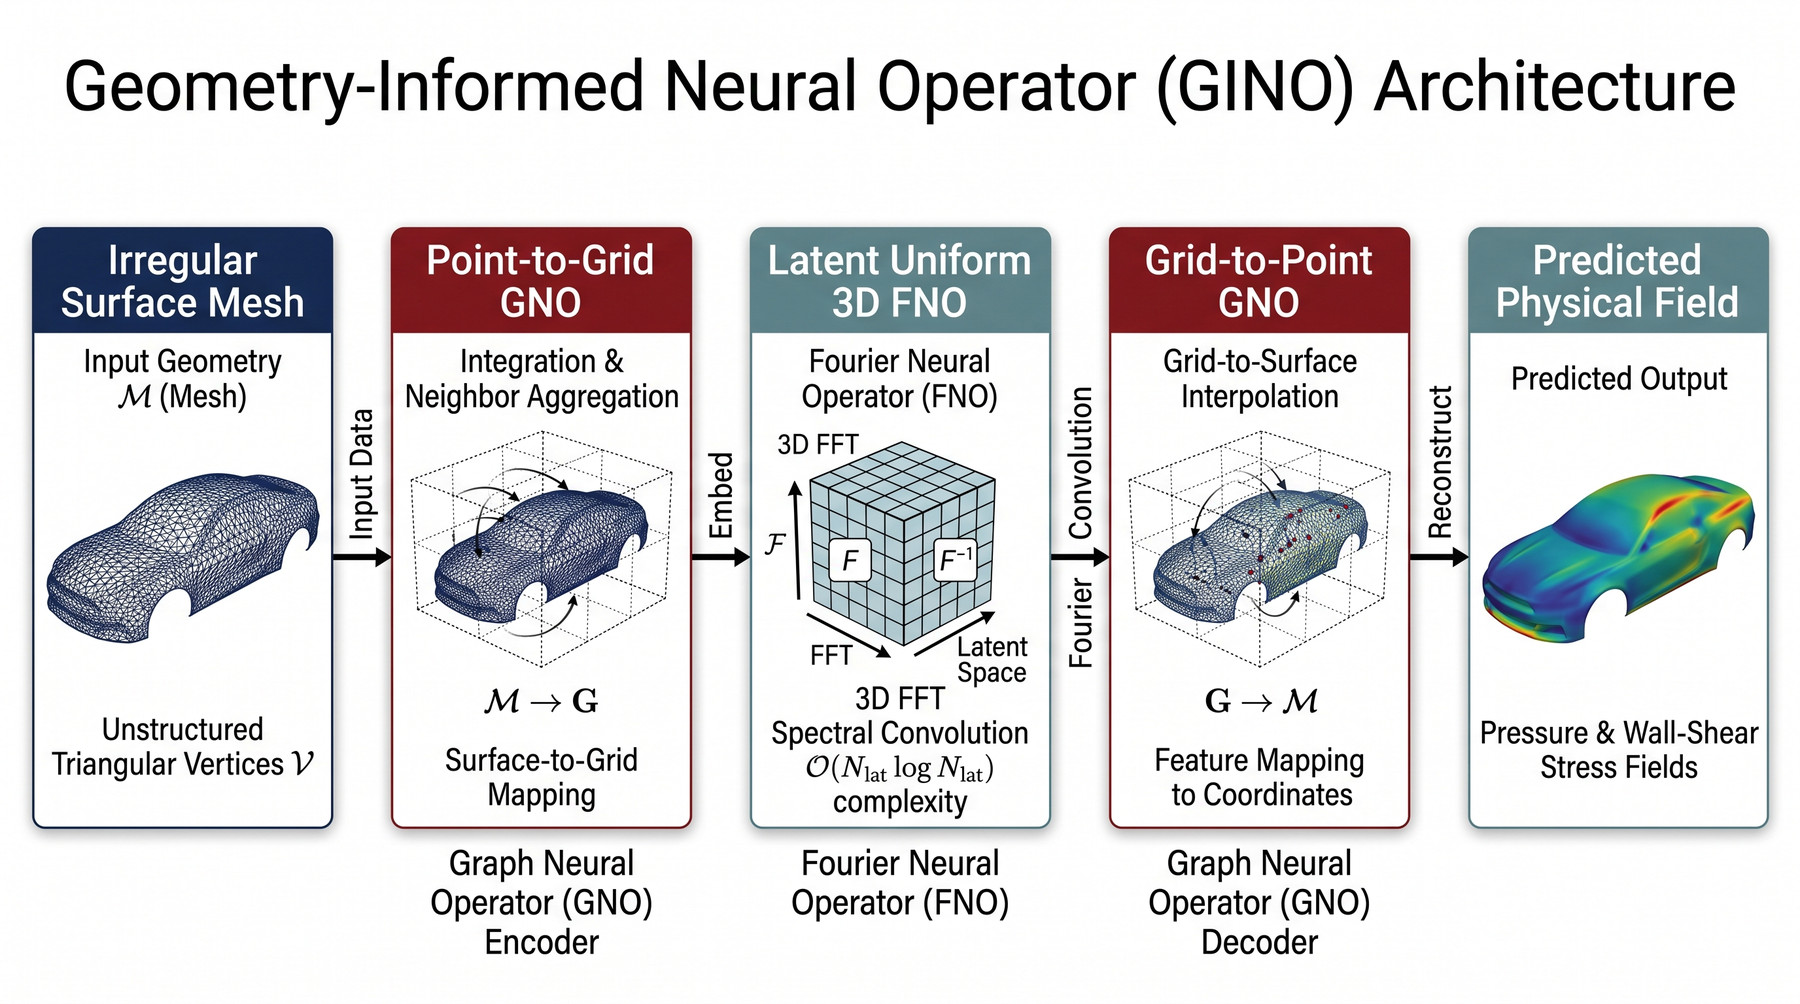
\includegraphics[width=0.92\textwidth]{fig_gino_pipeline.jpg}
\caption{\textbf{The Geometry-Informed Neural Operator (GINO) workflow.} An irregular surface mesh $\mathcal{M}_{\text{surf}}$ is projected onto a regular 3D latent bounding grid via a Point-to-Grid GNO layer. A fast 3D FNO processes latent features with $\mathcal{O}(N_{\text{lat}} \log N_{\text{lat}})$ spectral efficiency. Finally, a Grid-to-Point GNO decoder projects the processed latent state back to arbitrary surface evaluation coordinates.}
\label{fig:gino}
\end{figure}

The end-to-end pipeline operates in three distinct stages, and they are best described as one
quadrature, one transform stack, and the same quadrature run backwards. The
\textbf{point-to-grid encoder} integrates surface features $v_{\text{surf}}(x)$ onto a
regular, uniform latent grid $\Omega_{\text{latent}} \subset
\mathbb{R}^{H \times W \times D}$,
\index{point-to-grid projection}\index{Geometry-Informed Neural Operator (GINO)!pipeline stages}
\begin{equation}
  \label{eq:ch24-p2g}
  v_{\text{grid}}(z_k) = \sum_{x_j \in \mathcal{M}_{\text{surf}}} \kappa_{\text{enc}}(z_k - x_j)
  \, v_{\text{surf}}(x_j) \, w_j,
\end{equation}
where $z_k$ ranges over latent grid nodes and $w_j$ is again the tributary area of the surface
vertex $x_j$. Equation \eqref{eq:ch24-p2g} is \eqref{eq:ch24-gno-kernel} with the roles of
source and target interchanged, and the same sparsification choice: evaluated for every pair
$(z_k, x_j)$ the encoder costs $\Theta(N_{\text{lat}} N_{\text{surf}})$, which is precisely
the dense interaction \chapref{ch:part1-comparative-theoretical-taxonomy-of-archit} flags
beside \eqref{eq:ch8-gino}, so a workable implementation restricts the sum to surface points
within a radius of $z_k$ and recovers the edge-linear count. The
\textbf{latent operator processing} then applies stacked 3D Fourier neural operator layers to
$v_{\text{grid}}$; the structured layout is exactly $(B, C, H, W, D)$, and the layer is the
two-dimensional \texttt{SpectralConv2d} of
\chapref{ch:part2-fourier-neural-operators-fno-from-scratch} with one axis added --- a
real-input transform over three spatial axes in place of \texttt{rfft2}, the two-dimensional
real fast Fourier transform (FFT), a mode box that is a product of three contiguous index
ranges, \eqref{eq:ch05-modeset} read at $d=3$ rather than the planar $d=2$, and a contraction
written in
\texttt{einsum} notation (Einstein summation)\index{einsum contraction} with one index more.
Global communication in $\mathcal{O}(N_{\text{lat}} \log N_{\text{lat}})$ operations is what
that stage buys, and it is what the radius-$r$ layers cannot buy cheaply. The
\textbf{grid-to-point decoder} closes the pipeline by sampling the latent grid at the surface
evaluation coordinates,
\begin{equation}
  \label{eq:ch24-g2p}
  v_{\text{surf}}(x_i) = \sum_{z_k \in \mathcal{N}_r(x_i)} \kappa_{\text{dec}}(x_i - z_k) \,
  v_{\text{grid}}(z_k) \, \tilde{w}_k,
\end{equation}
which is \eqref{eq:ch24-p2g} read in the other direction: $\tilde{w}_k$ is now the cell volume
of the latent node rather than a surface dual area, and the output is indexed by the mesh, not
by the box. Because the evaluation points in \eqref{eq:ch24-g2p} are free arguments of the
decoder, the same trained weights return pressure and WSS on a tessellation that was never in
the training set --- the property that makes the construction a surrogate for a design sweep
rather than a predictor for a single part \cite{li2023geometry}.

Two further inputs carry geometry that the connectivity alone does not supply, and the two
layouts take them differently. On the mesh, the coordinates stay in the index structure rather
than becoming channels, exactly as \chapref{ch:part2-the-practitioner-s-paradigm-infinite-dimen}
found: they enter \eqref{eq:ch24-gno-kernel} as the displacement argument $x_i - x_j$, which is
how the \texttt{coords} tensor enters Listing~\ref{lst:gno-kernel-conv}. On the latent grid the
geometry has to become channels, and the field that does it is the signed distance function
(SDF) --- the distance from any point to the body's surface, negative inside
\index{signed distance function (SDF)}--- concatenated with the grid's own coordinates, so the
spectral operator can tell a solid from a void rather than inferring it from a sparse shell of
projected features. Without such an encoding, the interior of the bounding box is
indistinguishable from empty space and the burden of the geometry falls entirely on the two
graph interfaces.

Batching is where irregular geometry costs real engineering time. The structured layout of
\chapref{ch:part2-the-practitioner-s-paradigm-infinite-dimen}, $X \in
\mathbb{R}^{B \times C \times N_1 \times \cdots \times N_d}$, presumes that every sample
shares its shape, and the point-cloud layout $X_{\text{nodes}} \in
\mathbb{R}^{B \times N_{\text{nodes}} \times C}$ presumes that every mesh has the same node
count --- false the moment two bodies are compared.
\index{batching!irregular geometries}\index{point-cloud layout!ragged batches}Padding to the
largest mesh and masking the surplus edges works, but it converts raggedness into wasted
compute rather than removing it; per-sample loops with accumulated gradients keep memory
predictable and forfeit throughput; bucketing by node count splits the batch and complicates
the sampler. This is why the forward signature in Listing~\ref{lst:gno-kernel-conv} carries no
batch axis at all: it is one mesh per call. The GINO composition softens the problem rather
than solving it --- the ragged structure is confined to the encoder and decoder, while the
latent grid inside has a fixed shape that batches cleanly, which is a genuine advantage of
placing the expensive operator on a box.

% -----------------------------------------------------------------------------
\section{What Irregular Geometry Buys, and What It Costs}
\label{sec:ch24-ledger}
% -----------------------------------------------------------------------------

The comparison borrows three of the five axes
\chapref{ch:part1-comparative-theoretical-taxonomy-of-archit} fixes --- which class of kernels a
parameterization admits, what one query costs at a chosen resolution, and how strong a theorem
is attached to the class --- and leaves its other two, inductive bias and the relation between
parameter space and discretization, to the memory accounting and the refinement behavior below.
Against the FNO, on the first axis a graph layer keeps the kernel's
dependence on $a(x_i)$ and $a(x_j)$ and its support constraint in place of stationarity and
band-limiting, and it drops the requirement that the domain be a torus
\cite{kovachki2023neural,li2021fourier}. On the second axis it pays more: $\Theta(|E|\,
d_v^{2})$ per layer, quadratic in channel width on \emph{every} edge, against $\Theta(d_v N
\log N + K d_v^{2})$ for a spectral layer, where the quadratic term is confined to the $K$
retained modes. GINO's hybrid pays $\Theta(|E| + N_{\text{lat}} \log N_{\text{lat}})$ --- edge
work only at the interfaces --- but the latent box is a design parameter with a real floor:
$N_{\text{lat}} = HWD$ covers the bounding volume, so a slender body in a large box spends
most of its spectral budget on empty space, and the resolution needed to capture a thin
boundary layer sets the cost of the whole box. GNO and GINO
\index{Graph Neural Operator (GNO)!cost versus spectral layer}\index{Geometry-Informed Neural Operator (GINO)!cost of the latent box}
also differ from the FNO in what refinement touches. For the spectral operator the parameters
are mesh-free and one trained $\theta$ is queried at any $N$; for a graph operator the
parameters are mesh-free too, but the \emph{graph} is an input, so refinement changes $|E|$,
the memory footprint, and the realization of the layer rather than leaving $\theta$ alone
against a new grid. The third axis is the one on which honesty is cheapest: Part~I's ledger
Table~\ref{tab:ch8-ledger} records no universality statement, no rate, and no invariance proof
for either architecture, and the reason is visible in \eqref{eq:ch24-gno-kernel} --- a
radius-$r$ ball is a truncation of the kernel's support whose error is controlled by whatever
regularity the target has in the pair $(x,y)$, a question no theorem in this book answers.

What the geometry buys is scope rather than accuracy. It lets one trained operator serve a
parameterized family of bodies whose meshes differ in node count, connectivity, and spacing; it
lets the output be sampled wherever the engineer wants it rather than where the grid happens
to put nodes; and it retains the input-dependent kernel that inhomogeneous problems ask for.
The aerodynamic application, with its reported accuracy and its inference budget against a
volume solver, is taken up with the other large-scale 3D workloads in
\chapref{ch:part3-external-aerodynamics-and-surface-flows}. What it costs is edge-linear
computation with a quadratic channel factor, a memory footprint that scales with mesh size
rather than with parameters, an SDF and coordinate-channel pipeline that must be rebuilt for
every new computer-aided design tessellation, ragged batching at the two
interfaces, and the loss of every guarantee the spectral case enjoys.

One further obligation is procedural rather than architectural. The error split of
\eqref{eq:ch01-error-split} presupposed a discretization that was a refinement of one fixed
grid; here the graph is itself an argument of the layer. A reported error for a graph
surrogate is therefore a triple --- model, mesh, and metric --- and the protocol that makes it
readable evaluates the trained operator on the training tessellation, then on a
re-tessellation of the same body at different node density, and against a solver run on the
evaluation mesh rather than on the one the data came from. Where those three numbers diverge,
the divergence localizes in the quadrature of \eqref{eq:ch24-gno-kernel} --- in the weights,
the radius, or the depth needed to span the body --- a term the spectral construction can
leave implicit and this one cannot.

\takeaway{Graph Layers Are a Support Constraint, Not a New Family}{A GNO layer is the generic integral-kernel layer \eqref{eq:no_layer} with the kernel's support restricted to a radius-$r$ neighborhood and the mesh entering only through quadrature weights, so parameters stay mesh-free while the sum tracks the continuum integral. GINO confines that machinery to a point-to-grid encoder and a grid-to-point decoder and runs the global part of the operator on a latent grid, where a fast Fourier transform is legal and the mixing needs no depth to reach across the body. Neither construction restores a convergence guarantee.}

% -----------------------------------------------------------------------------

The three canonical problems that follow are chosen for the opposite reason. Burgers'
equation, Darcy flow, and the two-dimensional Navier--Stokes equations are posed on the
periodic torus or the unit square precisely so that a discrete Fourier transform is legal,
which makes them the controlled setting in which the spectral machinery of
\chapref{ch:part2-fourier-neural-operators-fno-from-scratch} can be judged without geometry in
the way \cite{li2021fourier}. \chapref{ch:part2-canonical-pde-benchmarks-and-reference-wor}
assembles those reference workflows: the input measures, the resolutions at which training and
evaluation grids differ, the relative-$L^{2}$ metric of
\chapref{ch:part2-the-practitioner-s-paradigm-infinite-dimen} that all three chapters share,
and the convergence behavior a practitioner should expect before tuning anything. Two of this
chapter's obligations carry forward there. The first is bookkeeping: an error number for a
graph operator must state the mesh it was measured on, since the mesh is part of the input
rather than an accident of the discretization. The second is methodological: the benchmarks
are where a reader can establish, on problems with a known answer, what the quadrature weights
and radius choices of \eqref{eq:ch24-gno-kernel} are supposed to accomplish before paying for
a latent box and a tessellated surface.
